\section{Introduction}
A standard sudoku is a puzzle containing a 9x9 grid. In each cell of the grid a number between 1 and 9 has to be placed in such a way that none of the rows and columns does contain duplicates numbers.
The main grid is divided is serveral subgrids of size 3x3. Those regions (typically indicated by a slightly ticker line) also cannot contain the same number twice. This paper extends the idea of a standard sudoku to a puzzle in 3 dimensions and investigates the complexity of those puzzles.

\begin{wrapfigure}{r}{4.5cm}

\begin{subfigure}[b]{0.55\textwidth}
   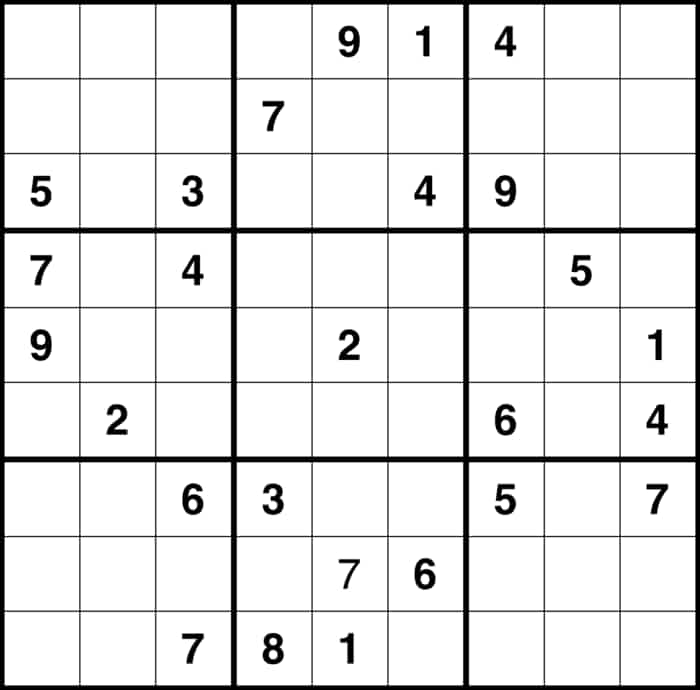
\includegraphics[width=4.5cm]{sudoku2d}

   \label{fig:Ng1} 
\end{subfigure}

\begin{subfigure}[b]{0.55\textwidth}
\vspace{.2cm}
   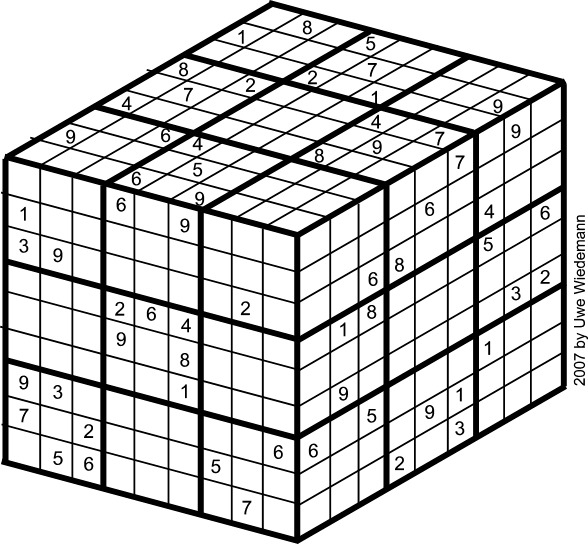
\includegraphics[width=4.5cm]{sudoku3d}

   \label{fig:Ng2}
\end{subfigure}

\end{wrapfigure} 

A 3D Sudoku is a Sudoku of size $N \times N \times N$. It consists of rows, columns, and layers, which are sequences of cells spanning across a single dimension. Similar to the 2D Sudoku, each row, column, and layer must contain every number $d \in \{1, \hdots, N\}$ exactly once. In contrast to 2D Sudokus, the constraint that every number must also appear exactly once in each block is dropped for the 3D Sudoku. 

Sudoku puzzles in newspaper and magazines mostly have one solution and involve no guessing This means that one could solve the puzzle by just applying logic rules. We will refer to those puzzles as deterministic puzzles. For a normal 2D sudoku the minimum number of givens is 17 \cite{sud16}. In this paper the relation between the size of the 3D sudoku and the relative number of given will be explored. As the size of the sudoku puzzle increases, the chance of bigger areas without sufficient information also increases. Based on this intuition our hypothesis is:  \textbf{As the size of a 3D sudoku grows, the relative number of givens needed to find a solution also increases.}